% This is samplepaper.tex, a sample chapter demonstrating the
% LLNCS macro package for Springer Computer Science proceedings;
% Version 2.20 of 2017/10/04
%
\documentclass[runningheads]{llncs}
%
\usepackage{amsmath}
\usepackage{booktabs} % For pretty tables
\usepackage{caption} % For caption spacing
\usepackage{subcaption} % For sub-figures
\usepackage{graphicx}
\usepackage{pgfplots}
\usepackage[all]{nowidow}
\usepackage[utf8]{inputenc}
\usepackage[margin=1in]{geometry}
\usepackage{tikz}
\usetikzlibrary{er,positioning,bayesnet}
\usepackage{multicol}
\usepackage{algpseudocode,algorithm,algorithmicx}
\usepackage{minted}
\usepackage{hyperref}
\usepackage{siunitx}
\usepackage[inline]{enumitem} % Horizontal lists
% Used for displaying a sample figure. If possible, figure files should
% be included in EPS format.
%
% If you use the hyperref package, please uncomment the following line
% to display URLs in blue roman font according to Springer's eBook style:
% \renewcommand\UrlFont{\color{blue}\rmfamily}

\newcommand{\card}[1]{\left\vert{#1}\right\vert}
\newcommand*\Let[2]{\State #1 $\gets$ #2}
\definecolor{blue}{HTML}{1F77B4}
\definecolor{orange}{HTML}{FF7F0E}
\definecolor{green}{HTML}{2CA02C}

\pgfplotsset{compat=1.14}

\renewcommand{\topfraction}{0.85}
\renewcommand{\bottomfraction}{0.85}
\renewcommand{\textfraction}{0.15}
\renewcommand{\floatpagefraction}{0.8}
\renewcommand{\textfraction}{0.1}
\setlength{\floatsep}{3pt plus 1pt minus 1pt}
\setlength{\textfloatsep}{3pt plus 1pt minus 1pt}
\setlength{\intextsep}{3pt plus 1pt minus 1pt}
\setlength{\abovecaptionskip}{2pt plus 1pt minus 1pt}

\begin{document}

\title{AER303 Aerospace Laboratory - Aerodynamic Forces on an Airfoil}
%\titlerunning{Add subtitle}

\author{Eric Dai\inst{1} \and Jai Willems\inst{2} \and Mingde Yin\inst{3}}
%\authorrunning{F. Author et al.}

\institute{Division of Engineering Science, University of Toronto, Toronto, Canada \email{eric.dai@mail.utoronto.ca}\\ \and Division of Engineering Science, University of Toronto, Toronto, Canada \email{jai.willems@mail.utoronto.ca}\\ \and Division of Engineering Science, University of Toronto, Toronto, Canada\\ \email{mingde.yin@mail.utoronto.ca}}

\maketitle


% -----------------------------------------------------------------------------
%   Abstract
% -----------------------------------------------------------------------------


\begin{abstract}

In this report the properties of the Clark Y airfoil are empirically explored at varying angles of attack by measuring airfoil surface and wake pressure distributions in a subsonic wind tunnel. The lift and drag are then calculated which are used to determine coefficients of lift, drag, and moment ($C_L$, $C_D$, and $C_M$, respectively). Measurements are collected using two separate methods, and their comparative effectiveness is evaluated.

\keywords{Airfoil \and Stall \and Inclined Manometer \and Scanivalve}
\end{abstract}


% -----------------------------------------------------------------------------
%   Nomenclature
% -----------------------------------------------------------------------------


\section*{Nomenclature}

This section defines useful terms and symbols for the purposes of this paper.

\begin{itemize}
    \item Voltage-pressure measurement: A measurement of the pressure calculated at a point in the wind tunnel in the voltage space as returned by the data acquisition card.
\end{itemize}


% -----------------------------------------------------------------------------
%   Introduction and Background
% -----------------------------------------------------------------------------


\section{Introduction and Background}\label{sec:introduction_and_background}

Airfoils are two-dimensional cross sections of wings which produce lift by redirecting flow over their surface such that the resulting surface pressure distribution causes a net upward force. At the same time, skin friction effects impart viscous drag forces on the airfoil. The combination of both the lift and drag forces impart a pitching moment on the airfoil. Lift, drag, and moment depend on the pressure distribution over the airfoil which will not remain constant over different angles of attack, and changes sharply near stall. Gaining insight into the angle of attack evolution of the airfoil's lift, drag, and moment is necessary for learning the stall and behavioural characteristics of the airfoil.

\subsection{Normal, Axial, and Moment Forces}

Ignoring viscous effects, the normal and axial forces on an airfoil describe the net effect of pressure on an airfoil. These forces yield lift and drag when combined with the angle of attack.

$P_u$ and $P_\ell$ are the pressure distributions over the airfoils top and bottom surfaces respectively, and $\theta$ is the clockwise angle between the chord normal and the airfoil surface normal.

The normal and axial forces acting on the airfoil are given by Equations \ref{eq:normal_force} and \ref{eq:axial_force}, integrating the pressure distribution over the surface to get the net forces where a positive value indicates forces acting upward normal to the chord and axially toward the trailing edge respectively. The moment around the leading edge of the airfoil is given by Equation \ref{eq:leading_edge_moment}, integrating the product of the moment arm and force acting in both the normal and axial direction. A positive value of $M_{LE}'$ pitches the airfoil up towards a higher angle of attack.

\begin{align}
    N' &= \int_{LE}^{TE} -P_u\cos\theta ds_u + \int_{LE}^{TE} P_\ell\cos\theta ds_\ell
    \label{eq:normal_force}\\
    A' &= \int_{LE}^{TE} -P_u\sin\theta ds_u + \int_{LE}^{TE} P_\ell\sin\theta ds_\ell
    \label{eq:axial_force}\\
    M' &= \int_{LE}^{TE} \left[(P_u\cos\theta)x - (P_u\sin\theta)y\right]ds_u + \int_{LE}^{TE} \left[(-P_\ell\cos\theta)x + (P_\ell\sin\theta)y\right]ds_\ell
    \label{eq:leading_edge_moment}
\end{align}

\subsection{Calculating Lift, Drag and Dimensionless Coefficients}

The lift of the airfoil is defined as the net force exerted on the airfoil normal to the relative airflow, whereas the drag is the net force exerted on the airfoil parallel to the relative airflow. These forces can be calculated using Equations \ref{eq:lift} and \ref{eq:drag} where the angle of attack, $\alpha$, is the angle between the airfoils chord line and the relative airflow.
\begin{align}
    L' &= N'\cos\alpha - A'\sin\alpha \label{eq:lift} \\
    D' &= N'\sin\alpha + A'\cos\alpha \label{eq:drag}
\end{align}

Lift, drag, and moment are nondimensionalized using Equations \ref{eq:cl}, \ref{eq:cd}, and \ref{eq:cm} respectively where\\
$q_\infty\equiv\frac{1}{2}\rho_\infty U_\infty^2$ is the freestream dynamic pressure and $C$ is the chord length.

\begin{align}
    C_L &= \frac{L'}{q_\infty C}
    \label{eq:cl}\\
    C_D &= \frac{D'}{q_\infty C}
    \label{eq:cd}\\
    C_M &= \frac{M'}{q_\infty C^2}
    \label{eq:cm}
\end{align}

\subsection{Stall}
Airfoil stall is characterized by a significant separation in flow from the airfoil surface resulting in loss of lift, increased drag, and a zero-or-positive pitching moment. Such conditions lead to unpredictable behaviour of an airfoil, and reduced aircraft controlability due to reduced effectiveness of aircrat control surfaces. It is important to understand the behaviour of a varying the angle of attack on the lift, drag, and moment characteristics of an airfoil to understand the limitations of the airfoil.

This report aims to explore the experimental performance of a Clark Y airfoil at varying angles of attack to understand the dependence of its performance characteristics on $\alpha$. A secondary goal of the report is to evaluate the comparative effectiveness of two methods of measuring pressure distributions.

%% TEST: Does a diagram like this look good?
\begin{figure}
    \centering
    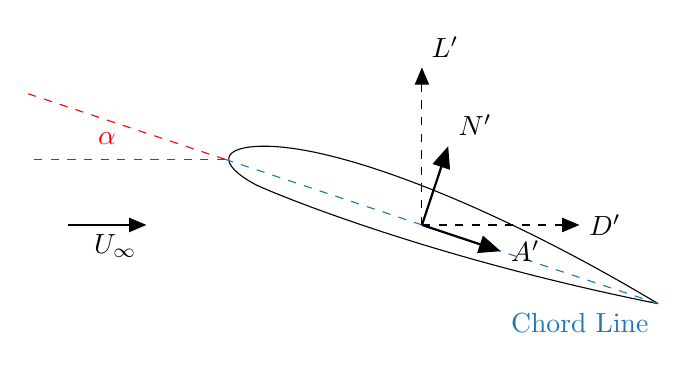
\begin{tikzpicture}
        \draw[rounded corners = 1cm] (6,-2)  .. controls (4, -0.8) and (2,0)  .. (0, 0) .. controls (1, -0.55) and (3, -1.4) .. (6,-2);
        \draw[dashed, blue] (0.5,-0.1666) -- (6,-2) node[anchor=north east] {Chord Line};
        \draw[dashed, red] (0.5,-0.1666) -- (-2,0.666);
        \draw[dashed, red] (0.5,-0.1666) -- (-2, -0.1666);
        \draw[red] (-1, 0.1) node {$\alpha$};
        \draw[->] (-1.5,-1) -- (-0.5,-1) node[anchor=north east] {$U_\infty$};
        \draw[thick,->] (3, -1) -- (3.3333, 0) node[anchor=south west] {$N'$};
        \draw[thick,->] (3, -1) -- (4, -1.333) node[anchor=west] {$A'$};
        \draw[dashed, ->] (3, -1) -- (3, 1) node[anchor=south west] {$L'$};
        \draw[dashed, ->] (3, -1) -- (5, -1) node[anchor=west] {$D'$};
    \end{tikzpicture}
    \caption{Definition of variables related to forces on an airfoil}
    \label{fig:airfoil_directions}
\end{figure}

% -----------------------------------------------------------------------------
%   Experimental Set-Up
% -----------------------------------------------------------------------------


\section{Experimental Set-Up}

This details the lab setup and experimental procedure used in the experiment.

\subsection{Apparatus}

\subsection{Procedure}

% What was measured and how was it aquired.

The procedure used for acquisition of pressure measurements was as follows:

\begin{enumerate}

    \item The first step in the experimental procedure is to determine the sample frequency and data acquisition time that allow for a $\pm 1\%$ accuracy in the pressure transducer measurements. We began by turning on the wind tunnel to a speed of $110\si{km}.\si{h}^{-1}$. We then took a series of representative measurements from the pressure transducer output with which we calculated the sample spectrum to determine the sample frequency and data acquisition time to use in the experiment.
    
    \item After calculating our sampling frequency and sampling time, we then determine the calibration curve that will allow us to transform the voltage-pressure representations gained from the pressure transducer into a useful pressure representation. To determine this correction curve, we varied the wind tunnel speed and took ten different voltage-pressure measurements using a MATLAB program and found the corresponding pressure measurements using the Betz manometer. This correspondance between representations can be used to calculate our pressure measurements in a useful representation.
    
    \item We then set the wind tunnel speed back to $110\si{km}.\si{h}^{-1}$ and measured the wind tunnel's pitot-static pressure difference to calculate the actual wind speed experiences in the wind tunnel.
    
    \item Next, we change the airfoil angle of attack in the positive and negative directions to determine the stall angle values. Using this information, we determined what angles of attack would be useful to measure such that we can accurately represent the airfoil properties up to and past stall conditions. The angle of attack values we chose were 0, 3, 6, 8, 10, 11, 13, 15, 16, 17, and 20 degrees.

    \item Cycling through each angle of attack, we measured the pressure distribution along the top and bottom surfaces of the airfoil in addition to the pressure distribution in the airfoils wake. These values were measured by reading the fluid hight changes from the inclined manometer. To get greater precision in the wake measurements, we moved the wake rake by $5\si{mm}$ and re-tookmeasurements again which increased our measurement density. Note that we took the measurements using two devices: (1) the pressure transducer controled by a MATLAB program and (2) an inclined manometer.

\end{enumerate}

Once the pressure measurements were taken, the data was pre-processed to get our pressure disstributions over the airfoil and in its wake. This pre-processing took different forms depending on the method used.

\begin{itemize}

    \item For data calculated using the pressure transducer, we used the calibration curve that provided a correspondance between the voltage-pressure representations gained from the pressure transducer and the pressure representations used in the experiment.

    \item For data calculated using the inclined manometer, we found the change of fluid height for each manometer tube compared to an "at-rest" state which and using Bernoulli's relation, determined the corresponding change in pressure.

\end{itemize}

After the data was pre-processed, the data was analyzed to determine the lift, moment, and drag coefficients as well as a measure of the lift, moment, and pressure drag of the airfoil up to and past the point of stall. The analysis was done using the methods described in section \ref{sec:introduction_and_background}.


% -----------------------------------------------------------------------------
%   Results and Discussion
% -----------------------------------------------------------------------------


\section{Results and Discussion}

\subsection{Comparison with XFOIL}

% -----------------------------------------------------------------------------
%   Conclusion
% -----------------------------------------------------------------------------


\section{Conclusion}


% -----------------------------------------------------------------------------
%   Bibliography
% -----------------------------------------------------------------------------


\bibliographystyle{ieeetr}
\bibliography{biblio}


% -----------------------------------------------------------------------------
%   Appendix
% -----------------------------------------------------------------------------


\appendix
\section{Pressure Measurements}


\end{document}
